\documentclass[]{article}
\usepackage{lmodern}
\usepackage{amssymb,amsmath}
\usepackage{ifxetex,ifluatex}
\usepackage{fixltx2e} % provides \textsubscript
\ifnum 0\ifxetex 1\fi\ifluatex 1\fi=0 % if pdftex
  \usepackage[T1]{fontenc}
  \usepackage[utf8]{inputenc}
\else % if luatex or xelatex
  \ifxetex
    \usepackage{mathspec}
    \usepackage{xltxtra,xunicode}
  \else
    \usepackage{fontspec}
  \fi
  \defaultfontfeatures{Mapping=tex-text,Scale=MatchLowercase}
  \newcommand{\euro}{€}
\fi
% use upquote if available, for straight quotes in verbatim environments
\IfFileExists{upquote.sty}{\usepackage{upquote}}{}
% use microtype if available
\IfFileExists{microtype.sty}{%
\usepackage{microtype}
\UseMicrotypeSet[protrusion]{basicmath} % disable protrusion for tt fonts
}{}
\usepackage[margin=1in]{geometry}
\usepackage{color}
\usepackage{fancyvrb}
\newcommand{\VerbBar}{|}
\newcommand{\VERB}{\Verb[commandchars=\\\{\}]}
\DefineVerbatimEnvironment{Highlighting}{Verbatim}{commandchars=\\\{\}}
% Add ',fontsize=\small' for more characters per line
\usepackage{framed}
\definecolor{shadecolor}{RGB}{248,248,248}
\newenvironment{Shaded}{\begin{snugshade}}{\end{snugshade}}
\newcommand{\KeywordTok}[1]{\textcolor[rgb]{0.13,0.29,0.53}{\textbf{{#1}}}}
\newcommand{\DataTypeTok}[1]{\textcolor[rgb]{0.13,0.29,0.53}{{#1}}}
\newcommand{\DecValTok}[1]{\textcolor[rgb]{0.00,0.00,0.81}{{#1}}}
\newcommand{\BaseNTok}[1]{\textcolor[rgb]{0.00,0.00,0.81}{{#1}}}
\newcommand{\FloatTok}[1]{\textcolor[rgb]{0.00,0.00,0.81}{{#1}}}
\newcommand{\CharTok}[1]{\textcolor[rgb]{0.31,0.60,0.02}{{#1}}}
\newcommand{\StringTok}[1]{\textcolor[rgb]{0.31,0.60,0.02}{{#1}}}
\newcommand{\CommentTok}[1]{\textcolor[rgb]{0.56,0.35,0.01}{\textit{{#1}}}}
\newcommand{\OtherTok}[1]{\textcolor[rgb]{0.56,0.35,0.01}{{#1}}}
\newcommand{\AlertTok}[1]{\textcolor[rgb]{0.94,0.16,0.16}{{#1}}}
\newcommand{\FunctionTok}[1]{\textcolor[rgb]{0.00,0.00,0.00}{{#1}}}
\newcommand{\RegionMarkerTok}[1]{{#1}}
\newcommand{\ErrorTok}[1]{\textbf{{#1}}}
\newcommand{\NormalTok}[1]{{#1}}
\usepackage{graphicx}
\makeatletter
\def\maxwidth{\ifdim\Gin@nat@width>\linewidth\linewidth\else\Gin@nat@width\fi}
\def\maxheight{\ifdim\Gin@nat@height>\textheight\textheight\else\Gin@nat@height\fi}
\makeatother
% Scale images if necessary, so that they will not overflow the page
% margins by default, and it is still possible to overwrite the defaults
% using explicit options in \includegraphics[width, height, ...]{}
\setkeys{Gin}{width=\maxwidth,height=\maxheight,keepaspectratio}
\ifxetex
  \usepackage[setpagesize=false, % page size defined by xetex
              unicode=false, % unicode breaks when used with xetex
              xetex]{hyperref}
\else
  \usepackage[unicode=true]{hyperref}
\fi
\hypersetup{breaklinks=true,
            bookmarks=true,
            pdfauthor={Lisa MALIPHOL},
            pdftitle={Exploratory Data Analysis MODBUS / TCP},
            colorlinks=true,
            citecolor=blue,
            urlcolor=blue,
            linkcolor=magenta,
            pdfborder={0 0 0}}
\urlstyle{same}  % don't use monospace font for urls
\setlength{\parindent}{0pt}
\setlength{\parskip}{6pt plus 2pt minus 1pt}
\setlength{\emergencystretch}{3em}  % prevent overfull lines
\setcounter{secnumdepth}{0}

%%% Use protect on footnotes to avoid problems with footnotes in titles
\let\rmarkdownfootnote\footnote%
\def\footnote{\protect\rmarkdownfootnote}

%%% Change title format to be more compact
\usepackage{titling}
\setlength{\droptitle}{-2em}
  \title{Exploratory Data Analysis\\MODBUS / TCP}
  \pretitle{\vspace{\droptitle}\centering\huge}
  \posttitle{\par}
  \author{Lisa MALIPHOL}
  \preauthor{\centering\large\emph}
  \postauthor{\par}
  \predate{\centering\large\emph}
  \postdate{\par}
  \date{June 2015}




\begin{document}

\maketitle


\section{Introduction}\label{introduction}

The following analysis was done using a pcap file created from a
simulation using the new SCADA simulation box under normal conditions
(no attacks):

capture\_sew\_20150617.pcap\\3.0 MB\\38,082 packets\\10 minutes

\section{Network Analysis}\label{network-analysis}

\subsection{Protocols}\label{protocols}

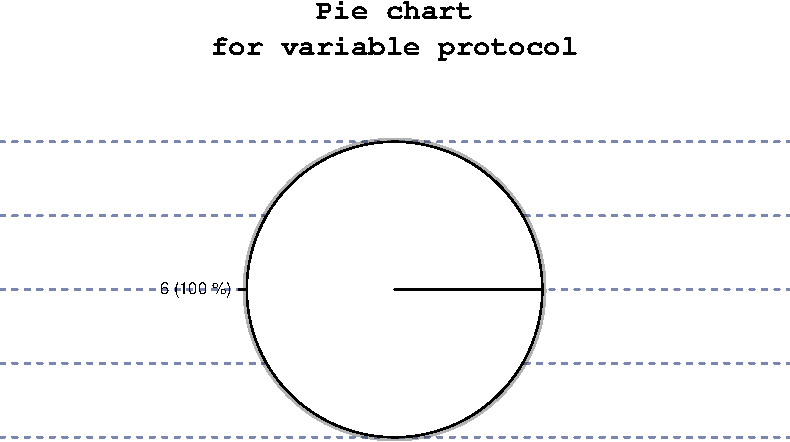
\includegraphics{modbus_files/figure-latex/unnamed-chunk-3-1.pdf}

\begin{center}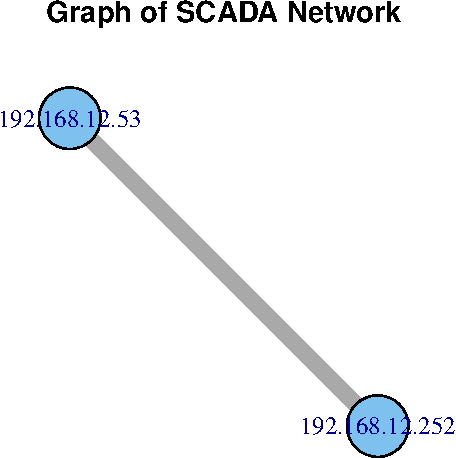
\includegraphics{modbus_files/figure-latex/warning-1} \end{center}

Source / Destination / UnitID

\begin{verbatim}
##            ip.src         ip.dst mbtcp.modbus.unit_id count
## 1:  192.168.12.53 192.168.12.252                    1 18496
## 2: 192.168.12.252  192.168.12.53                    1 18496
\end{verbatim}

Sources

\begin{verbatim}
##            ip.src count
## 1:  192.168.12.53 18496
## 2: 192.168.12.252 18496
\end{verbatim}

Destinations

\begin{verbatim}
##            ip.dst count
## 1: 192.168.12.252 18496
## 2:  192.168.12.53 18496
\end{verbatim}

Destination / UnitID

\begin{verbatim}
##            ip.dst mbtcp.modbus.unit_id count
## 1: 192.168.12.252                    1 18496
## 2:  192.168.12.53                    1 18496
\end{verbatim}

\begin{verbatim}
##            ip.src mbtcp.modbus.func_code count
## 1:  192.168.12.53                      4 18496
## 2: 192.168.12.252                      4 18496
\end{verbatim}

\section{Packet Analysis}\label{packet-analysis}

\begin{center}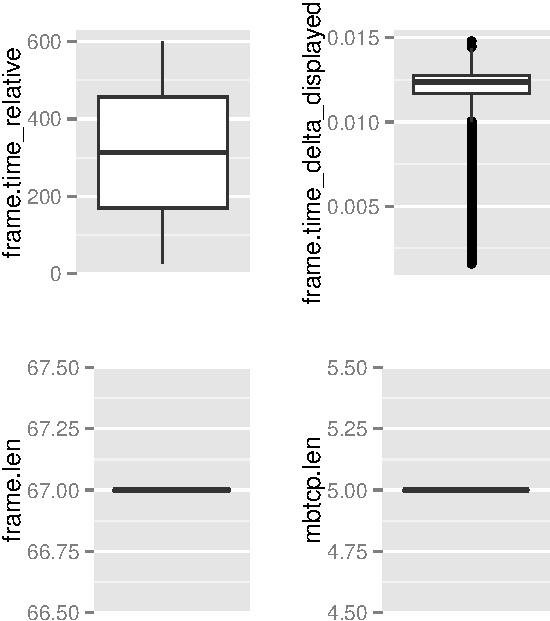
\includegraphics{modbus_files/figure-latex/unnamed-chunk-10-1} \end{center}

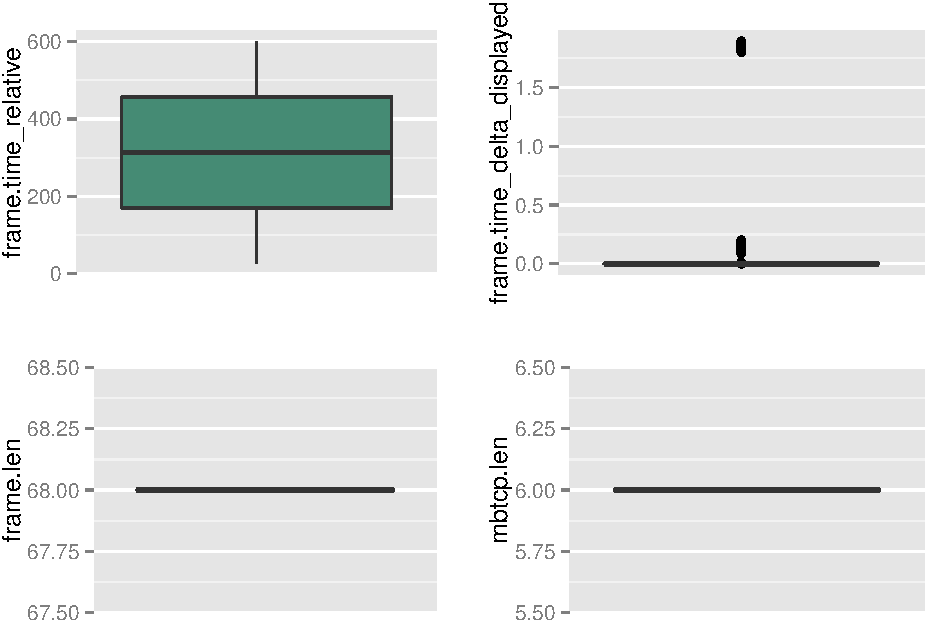
\includegraphics{modbus_files/figure-latex/unnamed-chunk-11-1.pdf}

\pagebreak

\subsection{MODBUS/TCP Request/Response Packet Statistics (Appendix
1)}\label{modbustcp-requestresponse-packet-statistics-appendix-1}

MODBUS/TCP \textbf{requests} are identified by packets having
destination port number 502

\begin{center}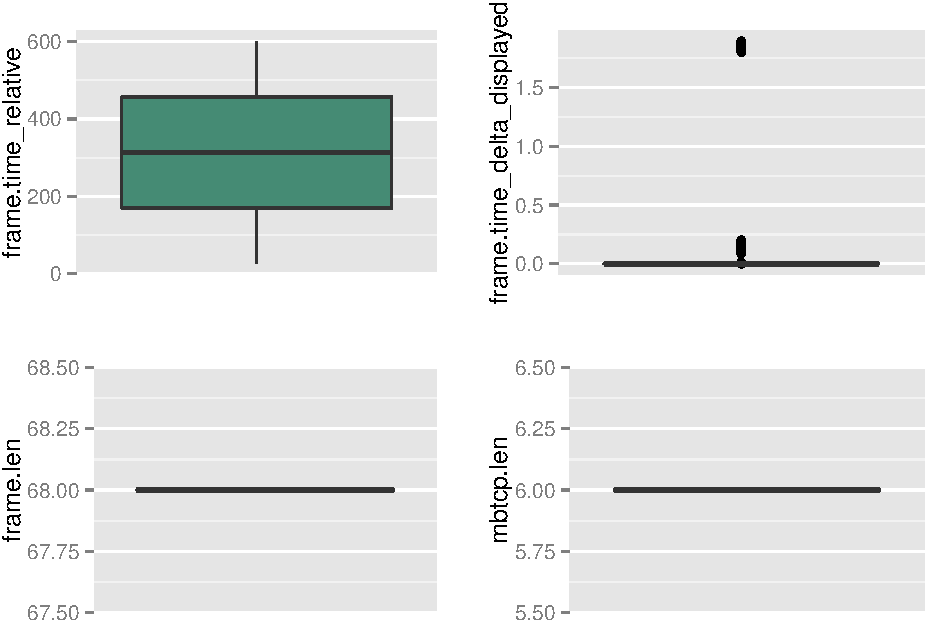
\includegraphics{modbus_files/figure-latex/unnamed-chunk-14-1} \end{center}

\pagebreak

MODBUS/TCP \textbf{responses} are identified by packets having source
port number 502

\begin{center}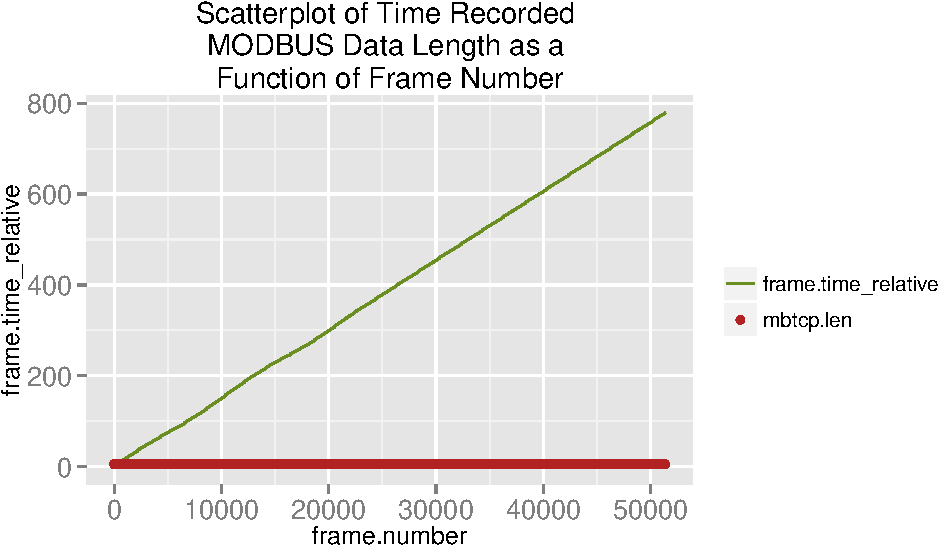
\includegraphics{modbus_files/figure-latex/unnamed-chunk-16-1} \end{center}

\pagebreak

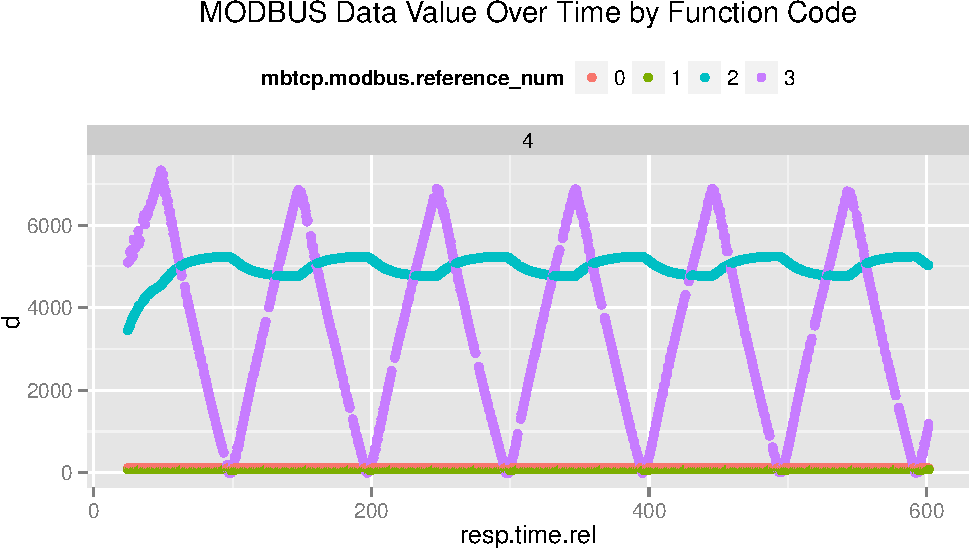
\includegraphics{modbus_files/figure-latex/unnamed-chunk-17-1.pdf}

\begin{center}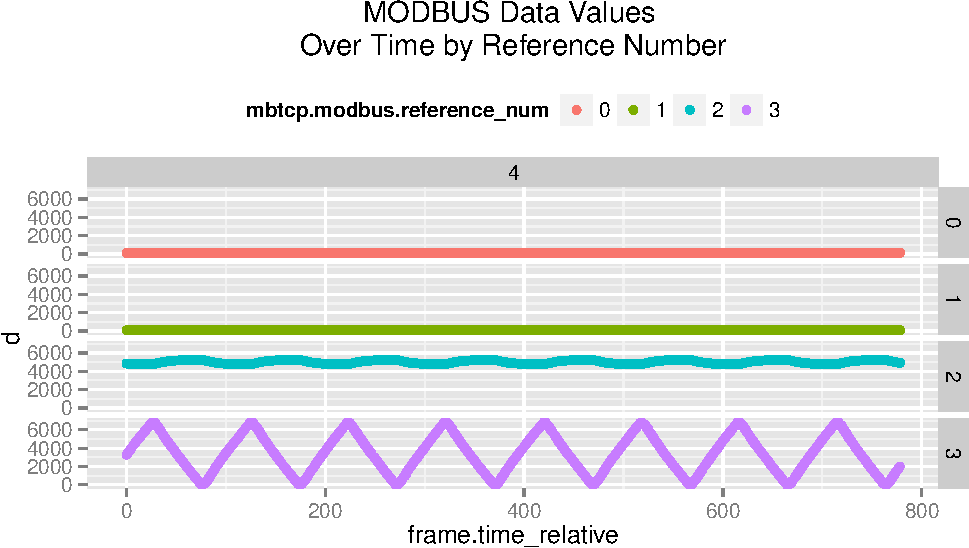
\includegraphics{modbus_files/figure-latex/unnamed-chunk-18-1} \end{center}

\pagebreak

\section[MODBUS/TCP Data Analysis]{MODBUS/TCP Data\footnote{\url{https://www.wireshark.org/docs/dfref/m/mbtcp.html}}
Analysis}\label{modbustcp-data1-analysis}

The following analysis was done over the previous dataset that has been
processed to merge response packet to the request packet of the same
transaction. An additional field ``d'' is the data field ``resp.data''
converted from a hex to a decimal value. (Appendix 2)
~\\\hspace*{0.333em}\\\hspace*{0.333em}

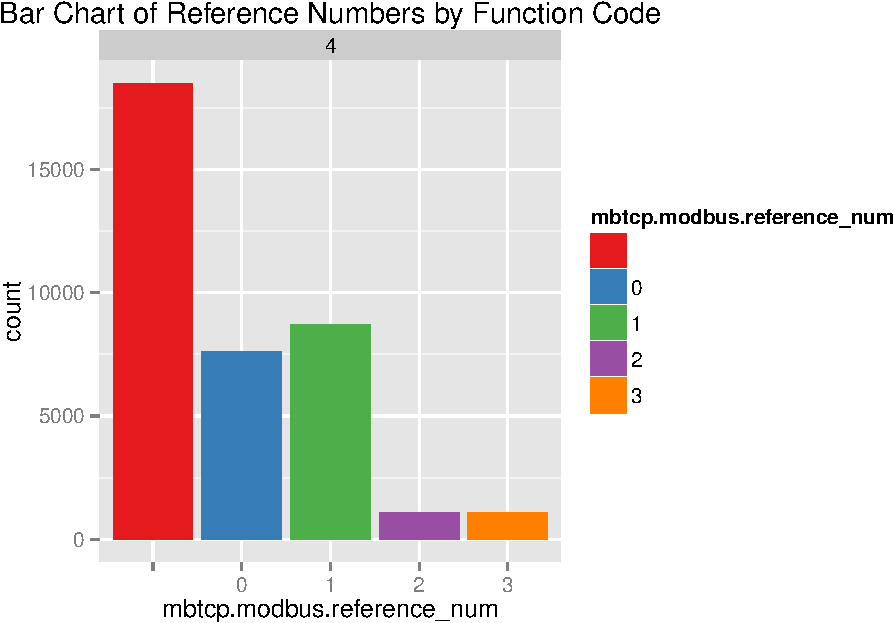
\includegraphics{modbus_files/figure-latex/unnamed-chunk-19-1.pdf}

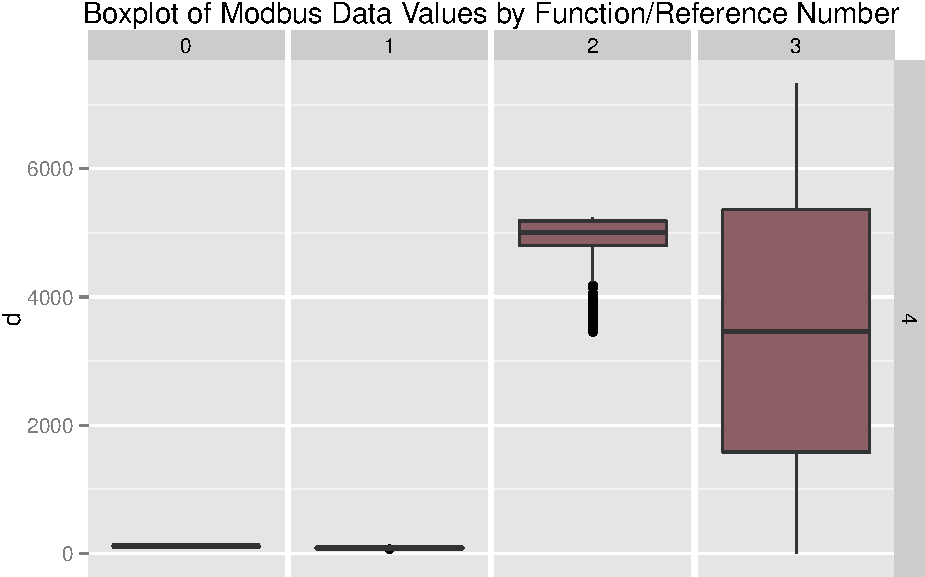
\includegraphics{modbus_files/figure-latex/unnamed-chunk-20-1.pdf}

\pagebreak

\section{MODBUS Data Value
Statistics}\label{modbus-data-value-statistics}

\begin{verbatim}
##    resp.func.code mbtcp.modbus.reference_num count d.min     d.mean d.max
## 1:              4                          0  7616   112  112.00000   112
## 2:              4                          1  8704    64   81.30423    84
## 3:              4                          2  1088  3455 4972.96140  5241
## 4:              4                          3  1088     0 3467.62592  7327
##           d.sd min.resp.time.rel min.resp.time.rel
## 1:    0.000000          24.53739          601.3492
## 2:    3.960659          24.58845          601.4262
## 3:  256.073630          24.52703          601.2214
## 4: 2125.525453          24.61349          601.3094
\end{verbatim}

\begin{center}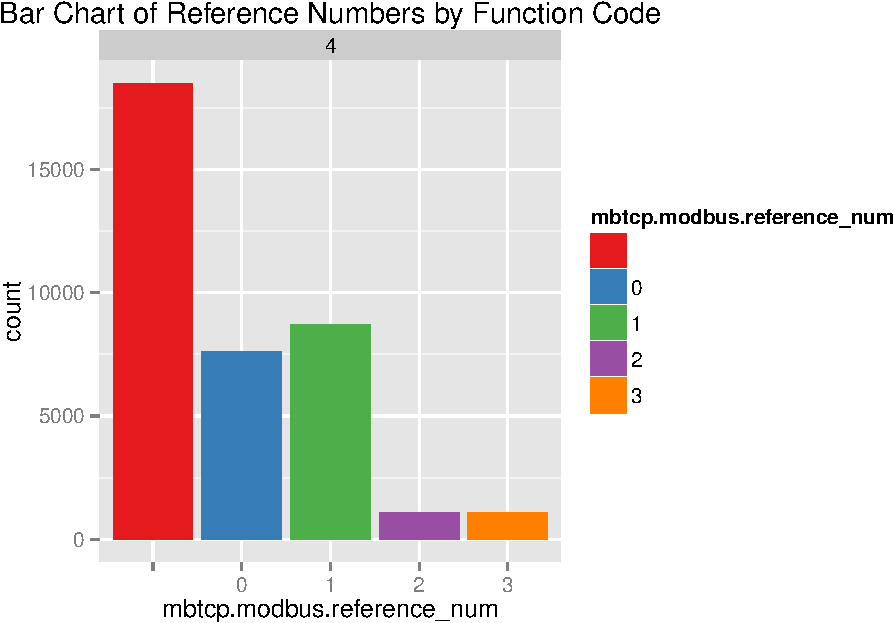
\includegraphics{modbus_files/figure-latex/unnamed-chunk-22-1} \end{center}

\pagebreak

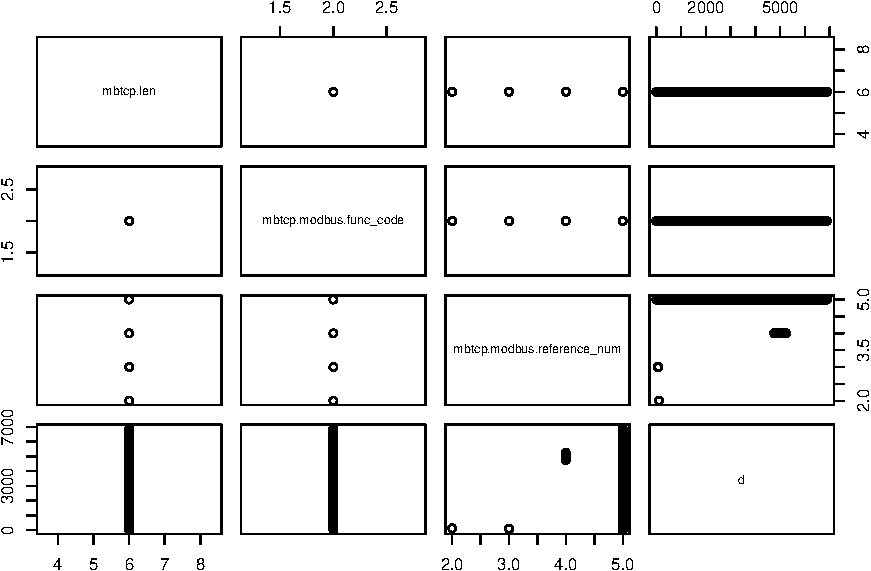
\includegraphics{modbus_files/figure-latex/unnamed-chunk-23-1.pdf}

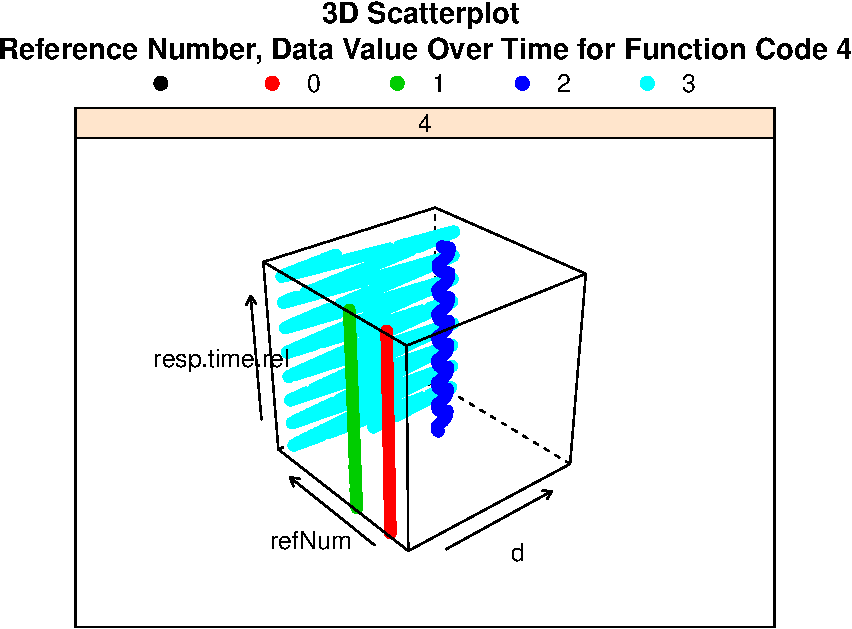
\includegraphics{modbus_files/figure-latex/unnamed-chunk-24-1.pdf}

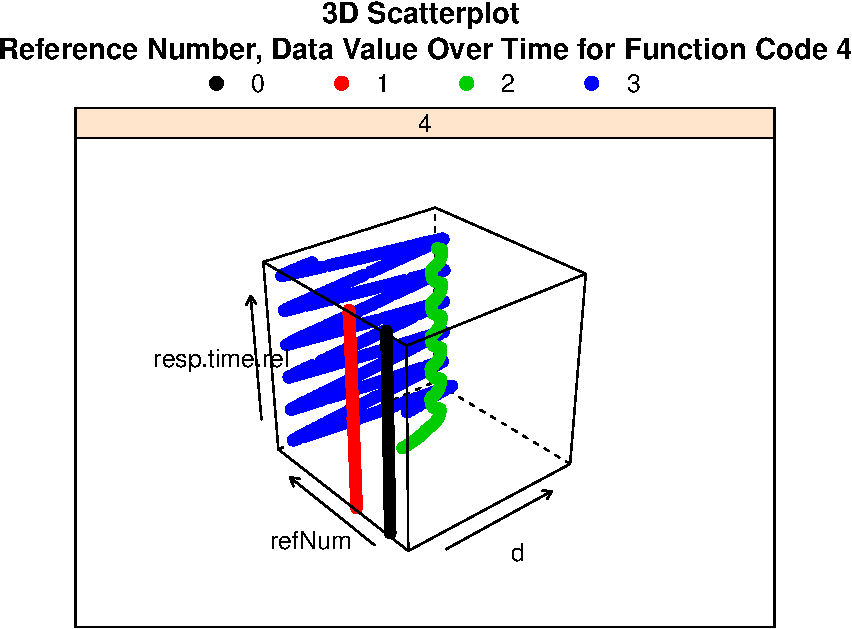
\includegraphics{modbus_files/figure-latex/unnamed-chunk-25-1.pdf}

\pagebreak

\section{Appendix 1 - MODBUS/TCP Request/Response Packet
Statistics}\label{appendix-1---modbustcp-requestresponse-packet-statistics}

\begin{Shaded}
\begin{Highlighting}[]
\KeywordTok{summary}\NormalTok{(requests)}
\end{Highlighting}
\end{Shaded}

\begin{verbatim}
##   frame.number   frame.time_relative frame.time_delta_displayed
##  Min.   :    5   Min.   : 24.52      Min.   :0.000162          
##  1st Qu.: 9524   1st Qu.:169.16      1st Qu.:0.000261          
##  Median :19044   Median :313.80      Median :0.000303          
##  Mean   :19044   Mean   :313.33      Mean   :0.009683          
##  3rd Qu.:28563   3rd Qu.:457.17      3rd Qu.:0.000355          
##  Max.   :38082   Max.   :601.41      Max.   :1.893315          
##    frame.len  ip.proto  ip.version            ip.src     
##  Min.   :68   6:18496   4:18496    192.168.12.252:    0  
##  1st Qu.:68                        192.168.12.53 :18496  
##  Median :68                                              
##  Mean   :68                                              
##  3rd Qu.:68                                              
##  Max.   :68                                              
##             ip.dst      mbtcp.modbus.unit_id tcp.srcport  tcp.dstport 
##  192.168.12.252:18496   Min.   :1            1058:18496   1058:    0  
##  192.168.12.53 :    0   1st Qu.:1            502 :    0   502 :18496  
##                         Median :1                                     
##                         Mean   :1                                     
##                         3rd Qu.:1                                     
##                         Max.   :1                                     
##  mbtcp.prot_id mbtcp.trans_id    mbtcp.len mbtcp.modbus.func_code
##   :    0       Min.   :  0.0   Min.   :6    :    0               
##  0:18496       1st Qu.: 64.0   1st Qu.:6   4:18496               
##                Median :127.0   Median :6                         
##                Mean   :127.4   Mean   :6                         
##                3rd Qu.:191.0   3rd Qu.:6                         
##                Max.   :255.0   Max.   :6                         
##  mbtcp.modbus.reference_num mbtcp.modbus.word_cnt mbtcp.modbus.data 
##   :   0                     Min.   :1             Length:18496      
##  0:7616                     1st Qu.:1             Class :character  
##  1:8704                     Median :1             Mode  :character  
##  2:1088                     Mean   :1                               
##  3:1088                     3rd Qu.:1                               
##                             Max.   :1
\end{verbatim}

\begin{Shaded}
\begin{Highlighting}[]
\KeywordTok{summary}\NormalTok{(responses)}
\end{Highlighting}
\end{Shaded}

\begin{verbatim}
##   frame.number   frame.time_relative frame.time_delta_displayed
##  Min.   :    6   Min.   : 24.53      Min.   :0.001583          
##  1st Qu.: 9525   1st Qu.:169.16      1st Qu.:0.011678          
##  Median :19044   Median :313.81      Median :0.012367          
##  Mean   :19044   Mean   :313.35      Mean   :0.011918          
##  3rd Qu.:28564   3rd Qu.:457.18      3rd Qu.:0.012762          
##  Max.   :38083   Max.   :601.43      Max.   :0.014795          
##                                                                
##    frame.len  ip.proto  ip.version            ip.src     
##  Min.   :67   6:18496   4:18496    192.168.12.252:18496  
##  1st Qu.:67                        192.168.12.53 :    0  
##  Median :67                                              
##  Mean   :67                                              
##  3rd Qu.:67                                              
##  Max.   :67                                              
##                                                          
##             ip.dst      mbtcp.modbus.unit_id tcp.srcport  tcp.dstport 
##  192.168.12.252:    0   Min.   :1            1058:    0   1058:18496  
##  192.168.12.53 :18496   1st Qu.:1            502 :18496   502 :    0  
##                         Median :1                                     
##                         Mean   :1                                     
##                         3rd Qu.:1                                     
##                         Max.   :1                                     
##                                                                       
##  mbtcp.prot_id mbtcp.trans_id    mbtcp.len mbtcp.modbus.func_code
##   :    0       Min.   :  0.0   Min.   :5    :    0               
##  0:18496       1st Qu.: 64.0   1st Qu.:5   4:18496               
##                Median :127.0   Median :5                         
##                Mean   :127.4   Mean   :5                         
##                3rd Qu.:191.0   3rd Qu.:5                         
##                Max.   :255.0   Max.   :5                         
##                                                                  
##  mbtcp.modbus.reference_num mbtcp.modbus.word_cnt mbtcp.modbus.data 
##   :18496                    Min.   : NA           Length:18496      
##  0:    0                    1st Qu.: NA           Class :character  
##  1:    0                    Median : NA           Mode  :character  
##  2:    0                    Mean   :NaN                             
##  3:    0                    3rd Qu.: NA                             
##                             Max.   : NA                             
##                             NA's   :18496
\end{verbatim}

\pagebreak

\section{Appendix 2 - Merged Request/Response Packet
Statistics}\label{appendix-2---merged-requestresponse-packet-statistics}

\begin{Shaded}
\begin{Highlighting}[]
\KeywordTok{summary}\NormalTok{(mergedSewDT)}
\end{Highlighting}
\end{Shaded}

\begin{verbatim}
##   frame.number   frame.time_relative frame.time_delta_displayed
##  Min.   :    5   Min.   : 24.52      Min.   :0.000162          
##  1st Qu.: 9524   1st Qu.:169.16      1st Qu.:0.000261          
##  Median :19044   Median :313.80      Median :0.000303          
##  Mean   :19044   Mean   :313.33      Mean   :0.009683          
##  3rd Qu.:28563   3rd Qu.:457.17      3rd Qu.:0.000355          
##  Max.   :38082   Max.   :601.41      Max.   :1.893315          
##                                                                
##    frame.len            ip.src                 ip.dst     
##  Min.   :68   192.168.12.53:18496   192.168.12.252:18496  
##  1st Qu.:68                                               
##  Median :68                                               
##  Mean   :68                                               
##  3rd Qu.:68                                               
##  Max.   :68                                               
##                                                           
##  mbtcp.modbus.unit_id tcp.srcport  tcp.dstport mbtcp.prot_id
##  1:18496              1058:18496   502:18496   0:18496      
##                                                             
##                                                             
##                                                             
##                                                             
##                                                             
##                                                             
##  mbtcp.trans_id    mbtcp.len mbtcp.modbus.func_code mbtcp.modbus.word_cnt
##  Min.   :  0.0   Min.   :6   4:18496                Min.   :1            
##  1st Qu.: 64.0   1st Qu.:6                          1st Qu.:1            
##  Median :127.0   Median :6                          Median :1            
##  Mean   :127.4   Mean   :6                          Mean   :1            
##  3rd Qu.:191.0   3rd Qu.:6                          3rd Qu.:1            
##  Max.   :255.0   Max.   :6                          Max.   :1            
##                                                                          
##  mbtcp.modbus.reference_num resp.fr.number  resp.time.rel   
##  0:7616                     Min.   :    6   Min.   : 24.53  
##  1:8704                     1st Qu.: 9525   1st Qu.:169.16  
##  2:1088                     Median :19044   Median :313.81  
##  3:1088                     Mean   :19044   Mean   :313.35  
##                             3rd Qu.:28564   3rd Qu.:457.18  
##                             Max.   :38083   Max.   :601.43  
##                                                             
##  resp.time.delta       resp.len            resp.src    
##  Min.   :0.001583   Min.   :67   192.168.12.252:18496  
##  1st Qu.:0.011678   1st Qu.:67                         
##  Median :0.012367   Median :67                         
##  Mean   :0.011918   Mean   :67                         
##  3rd Qu.:0.012762   3rd Qu.:67                         
##  Max.   :0.014795   Max.   :67                         
##                                                        
##          resp.dest     resp.srcport resp.dstport resp.prot_id
##  192.168.12.53:18496   502:18496    1058:18496   0:18496     
##                                                              
##                                                              
##                                                              
##                                                              
##                                                              
##                                                              
##  resp.trans_id   resp.mbcp.len resp.func.code   resp.data   
##  Min.   :  0.0   Min.   :5     4:18496        00:70  :7616  
##  1st Qu.: 64.0   1st Qu.:5                    00:50  :4212  
##  Median :127.0   Median :5                    00:54  :4162  
##  Mean   :127.4   Mean   :5                    00:40  : 331  
##  3rd Qu.:191.0   3rd Qu.:5                    14:74  :  21  
##  Max.   :255.0   Max.   :5                    14:70  :  15  
##                                               (Other):2139  
##        d         
##  Min.   :   0.0  
##  1st Qu.:  84.0  
##  Median : 112.0  
##  Mean   : 580.9  
##  3rd Qu.: 112.0  
##  Max.   :7327.0  
## 
\end{verbatim}

\section{Appendix 3 - Commands and
Scripts}\label{appendix-3---commands-and-scripts}

\subsection{TShark}\label{tshark}

Command used to extract various fields from the pcap file used for
analysis.

tshark -r modbus.pcap -T fields -E separator=, -t r -E header=y -e
frame.number -e frame.time\_relative -e frame.time\_delta\_displayed -e
frame.len -e ip.proto -e ip.version -e ip.src -e eth.src -e ip.dst -e
eth.dst -e mbtcp.modbus.unit\_id -e tcp.srcport -e tcp.dstport -e
mbtcp.prot\_id -e mbtcp.trans\_id -e mbtcp.len -e
mbtcp.modbus.func\_code -e mbtcp.modbus.reference\_num -e
mbtcp.modbus.word\_cnt -e mbtcp.modbus.data \textgreater{} modbus.data

\subsection{sed}\label{sed}

Command used to remove empty lines from the pcap data.

sed '/\^{},,,,,.*\$/d' modbus.data \textgreater{} modbus.data

\subsection{R}\label{r}

install.R - Setup script to install required packages. sewModbus.R -
Script for processing, analysing and visualizing modbus data.

\end{document}
